
	This work proposes to compare four interfaces for the command of the iCub robot: a \ac{GUI}, a \ac{DPad}, a \ac{Wiimote} device, and a Kinect device.
	
	The interactions can be made with two different control methods either at the single motor level, or Cartesian level. The single motor control is done by setting the angle value of each motor individually. The Cartesian control uses inverse kinematics to define how a set of motors should be positioned so that an end-effector reaches its goal.
	
	\begin{figure}[htb]
	\begin{center}
	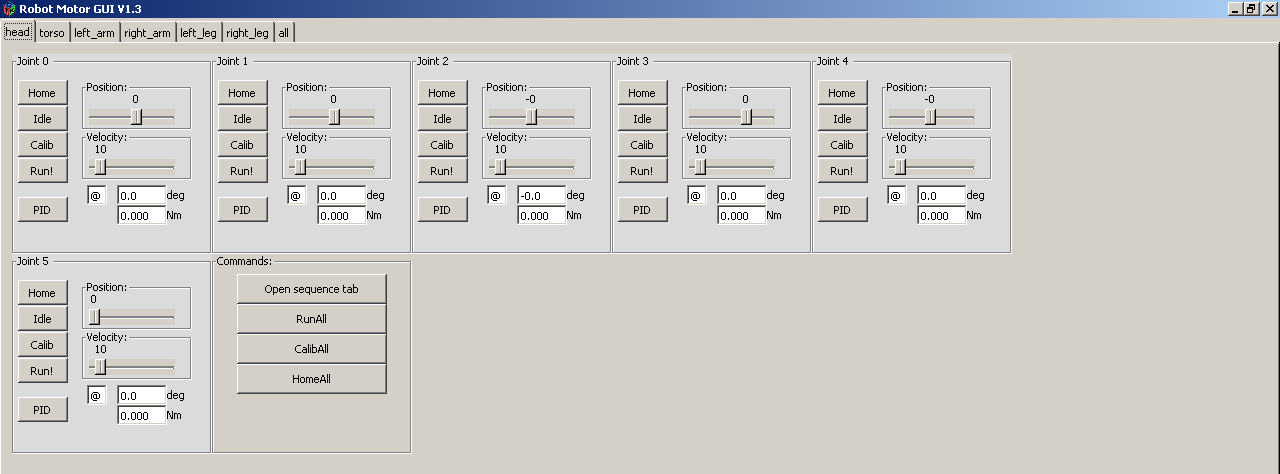
\includegraphics[width=70mm]{robotMotorGui.png}
	\end{center}
	\caption[Computer motor interface]{Computer motor interface - named robotMotorGui.} 
	\label{fig:robotMotorGui}
	\end{figure}
	
	The \ac{GUI} interface, shown in figure \ref{fig:robotMotorGui}, was already available in the iCub repository, so no development was needed. This interface has implemented a single motor and a Cartesian control, although in this work only the Cartesian control is used. This option was taken because the motor control with the \ac{GUI} interface was too complex. To define the goal 3D point of the end-effector the \ac{GUI} interface has three sliders, one slider per axis. Altering the position of the sliders will alter the desired position of the end-effector. Through this interface it is possible, also by the mean of sliders, to define the amount of time to reach the desired position from the current point, and the orientation of the end-effector. There can be only one slider altered at a time, each time that a slider is altered the user must wait until the end-effector reaches the desired position.
	
	The \ac{DPad} interface uses the \ac{Wiimote} buttons, although its functionality could be easily passed to a computer or any other device with six programmable buttons. The front, back, left, and right buttons, move the robot end-effector in the same height plane in the respective directions relatively to the iCub robot. To alter the height of the end-effector the - and + buttons of the remote can be used, moving it down and up respectively. The robot only moves while the user is pressing in one of the buttons. The movements allowed by this interface are illustrated in figure \ref{fig:dpadControl}.
	
	\begin{figure}[htb]
	\begin{center}
	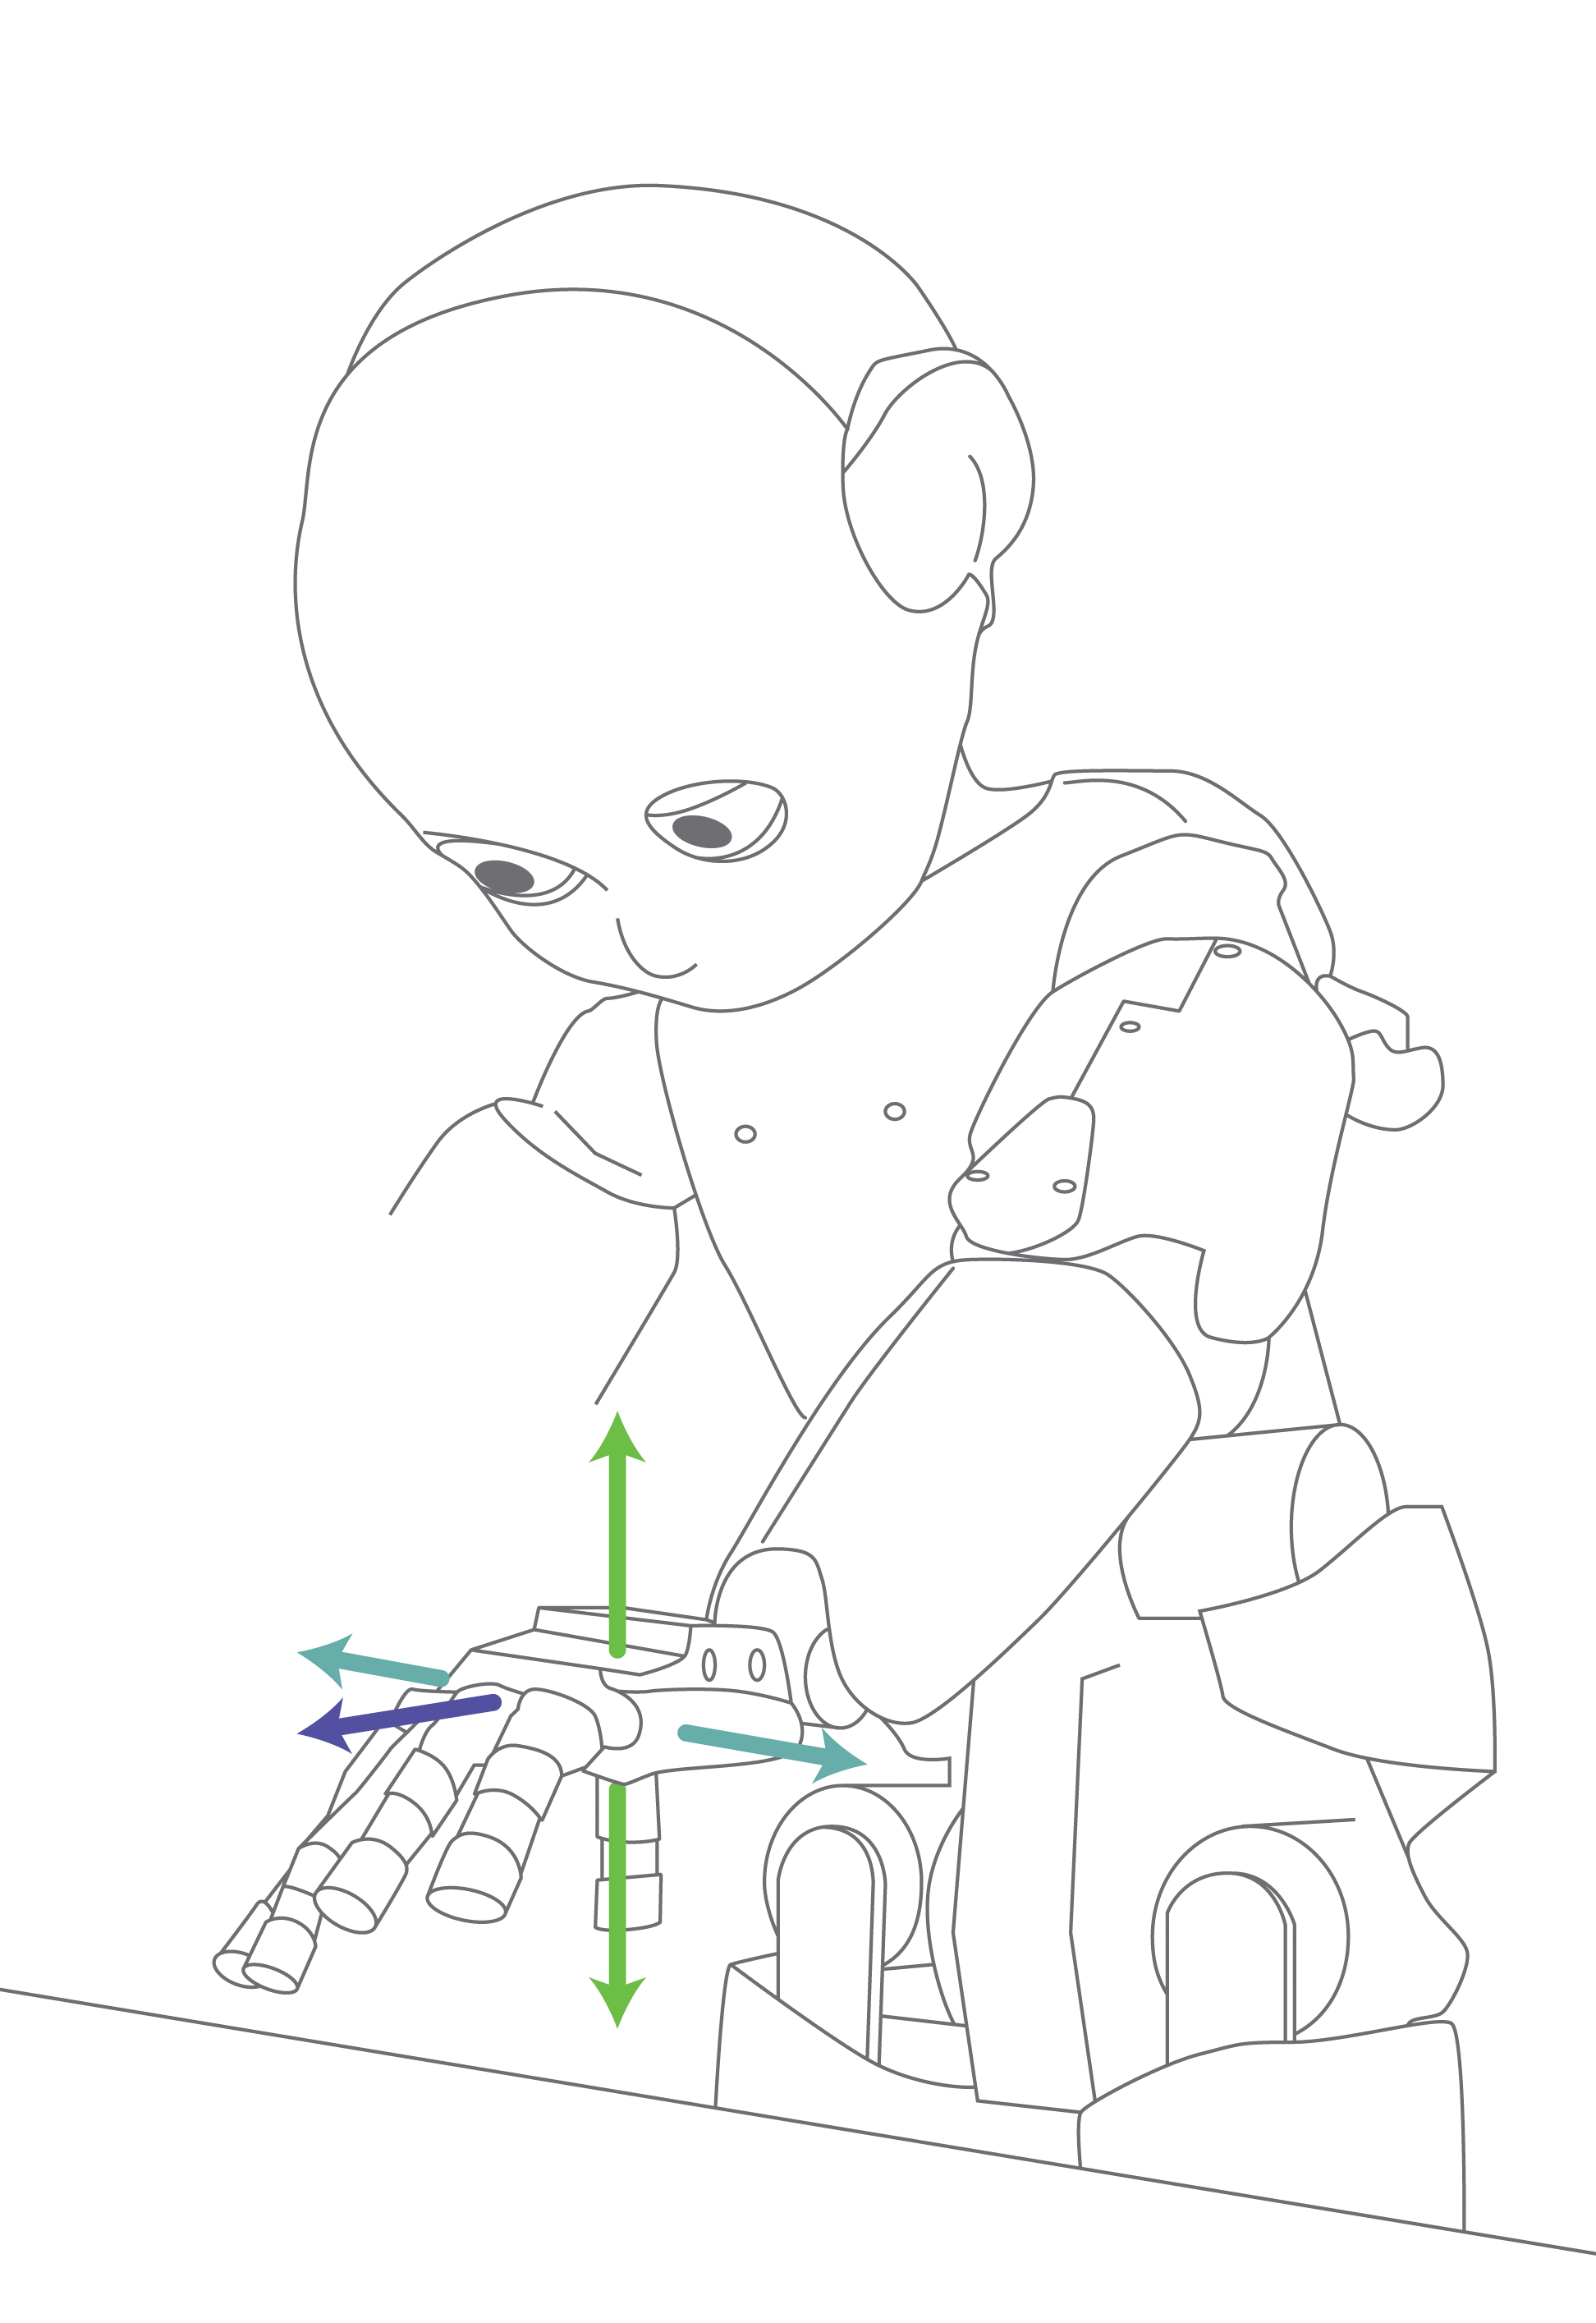
\includegraphics[width=34mm]{icubWiimoteCursor.png}
	\end{center}
	\caption[\ac{DPad} control type]{\ac{DPad} interface movements.} 
	\label{fig:dpadControl}
	\end{figure}
	
	The \ac{Wiimote} and Kinect interfaces were both developed specifically for this work. All of these interfaces only work while the trigger button (button B) on the bottom of the \ac{Wiimote} is pressed. This button has no other use than setting the control on and off in both interfaces.
	
	\begin{figure}[htb]
	\begin{center}
	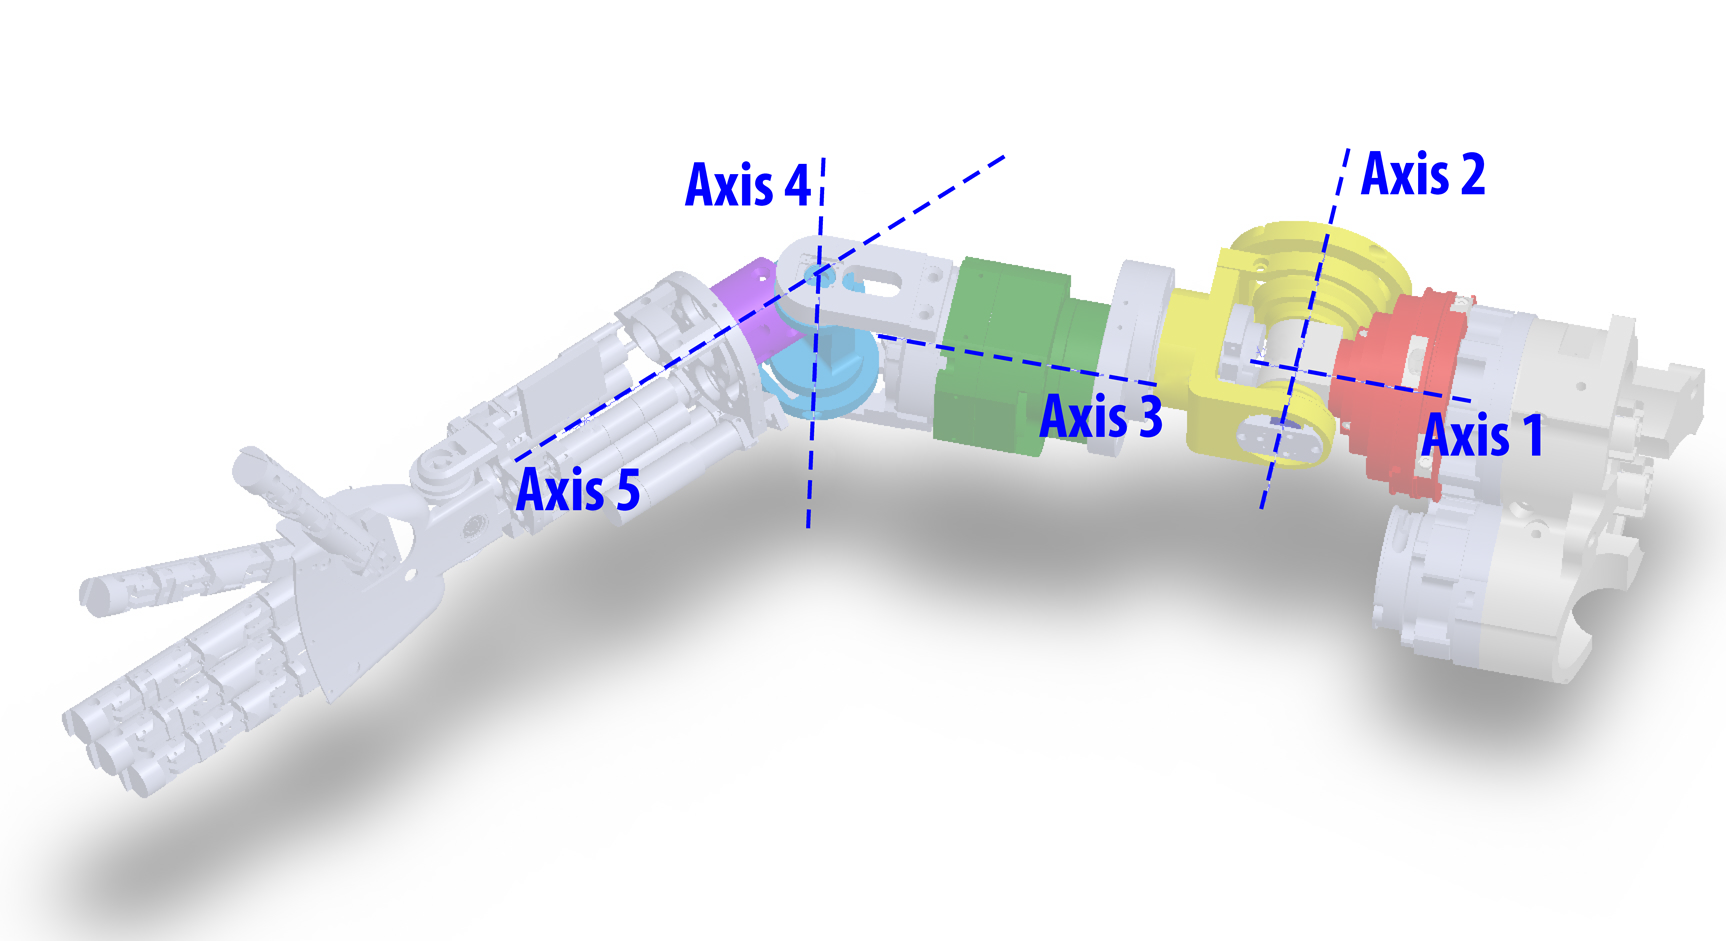
\includegraphics[width=70mm]{icubArm.png}
	\end{center}
	\caption[\ac{Wiimote} controlled motors in the iCub arm]{\ac{Wiimote} controlled motors in the iCub arm.} 
	\label{fig:icubArm}
	\end{figure}
	
	The \ac{Wiimote} motor control maps the rotation made around each axis to a different motor. Because there are more motors to be controlled in the iCub arm than rotation axis, the arm is divided into two parts. The arm and the forearm, the selection of which part to control can be made by pressing buttons one and two. The angle of a motor only changes while the user is rotating the remote around the intended axis, when the user stops moving the \ac{Wiimote} the robot stops immediately. The motors controlled and the axis of each motor are shown in figure \ref{fig:icubArm}. In figure \ref{fig:wiiMotorControl} the arrows show the type of rotation per each part, blue arrows arm part, orange arrows forearm part.
	
	The \ac{Wiimote} kinematic control is mapped to the rotations of the arm around the iCub shoulder with a constant radius. The radius can be altered by pressing the - and + buttons, that decrease or increase the radius size. What is meant by this explanation is that the end-effector always follows a virtual point that is controlled by the \ac{Wiimote}. That virtual point rotates around an origin point, the shoulder, from which maintains a constant distance. A rotation of the \ac{Wiimote} around its X axis, results in a rotation of the virtual point with the same amount of degrees around the origin point in the X axis. In figure \ref{fig:wiiCartesianControl} the yellow line represents the radius, the brown ball represents the end-effector.
	
		\begin{figure}[htb]
	\centering
	  \subfloat[Motor control.]{\label{fig:wiiMotorControl}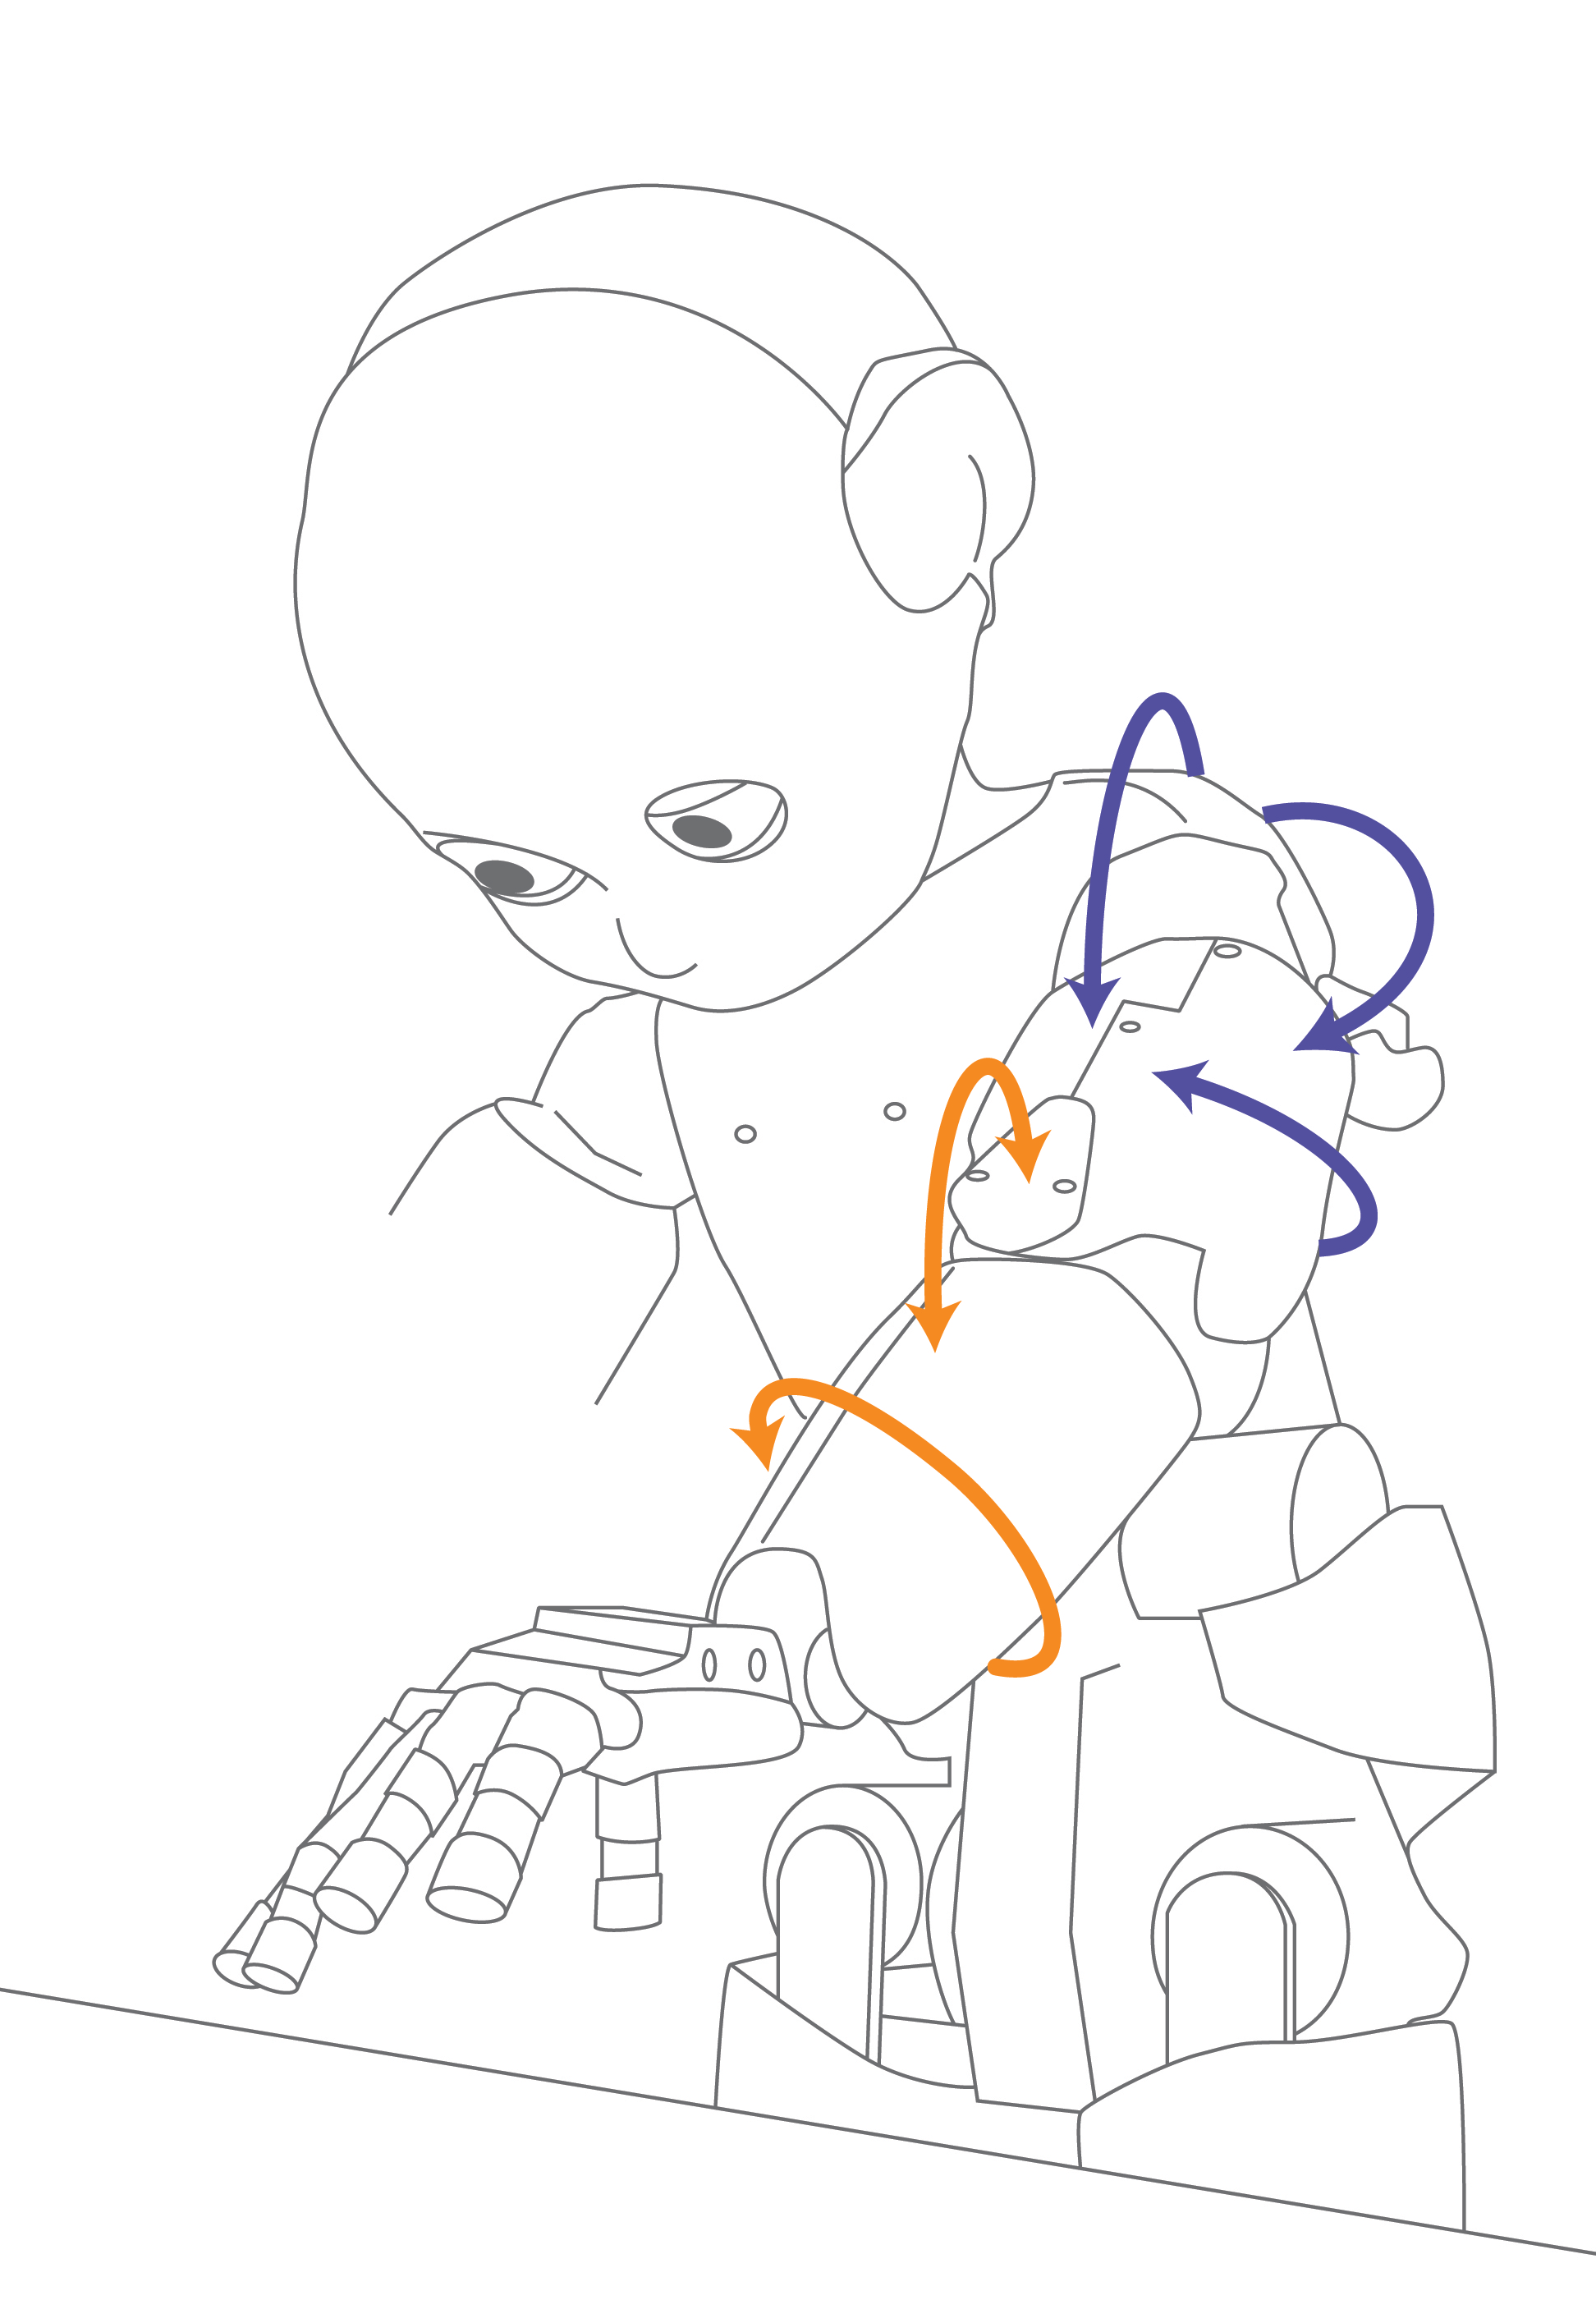
\includegraphics[width=34mm]{icubWiimoteMotor.png}}
  \hspace{5mm}
	  \subfloat[Cartesian control.]{\label{fig:wiiCartesianControl}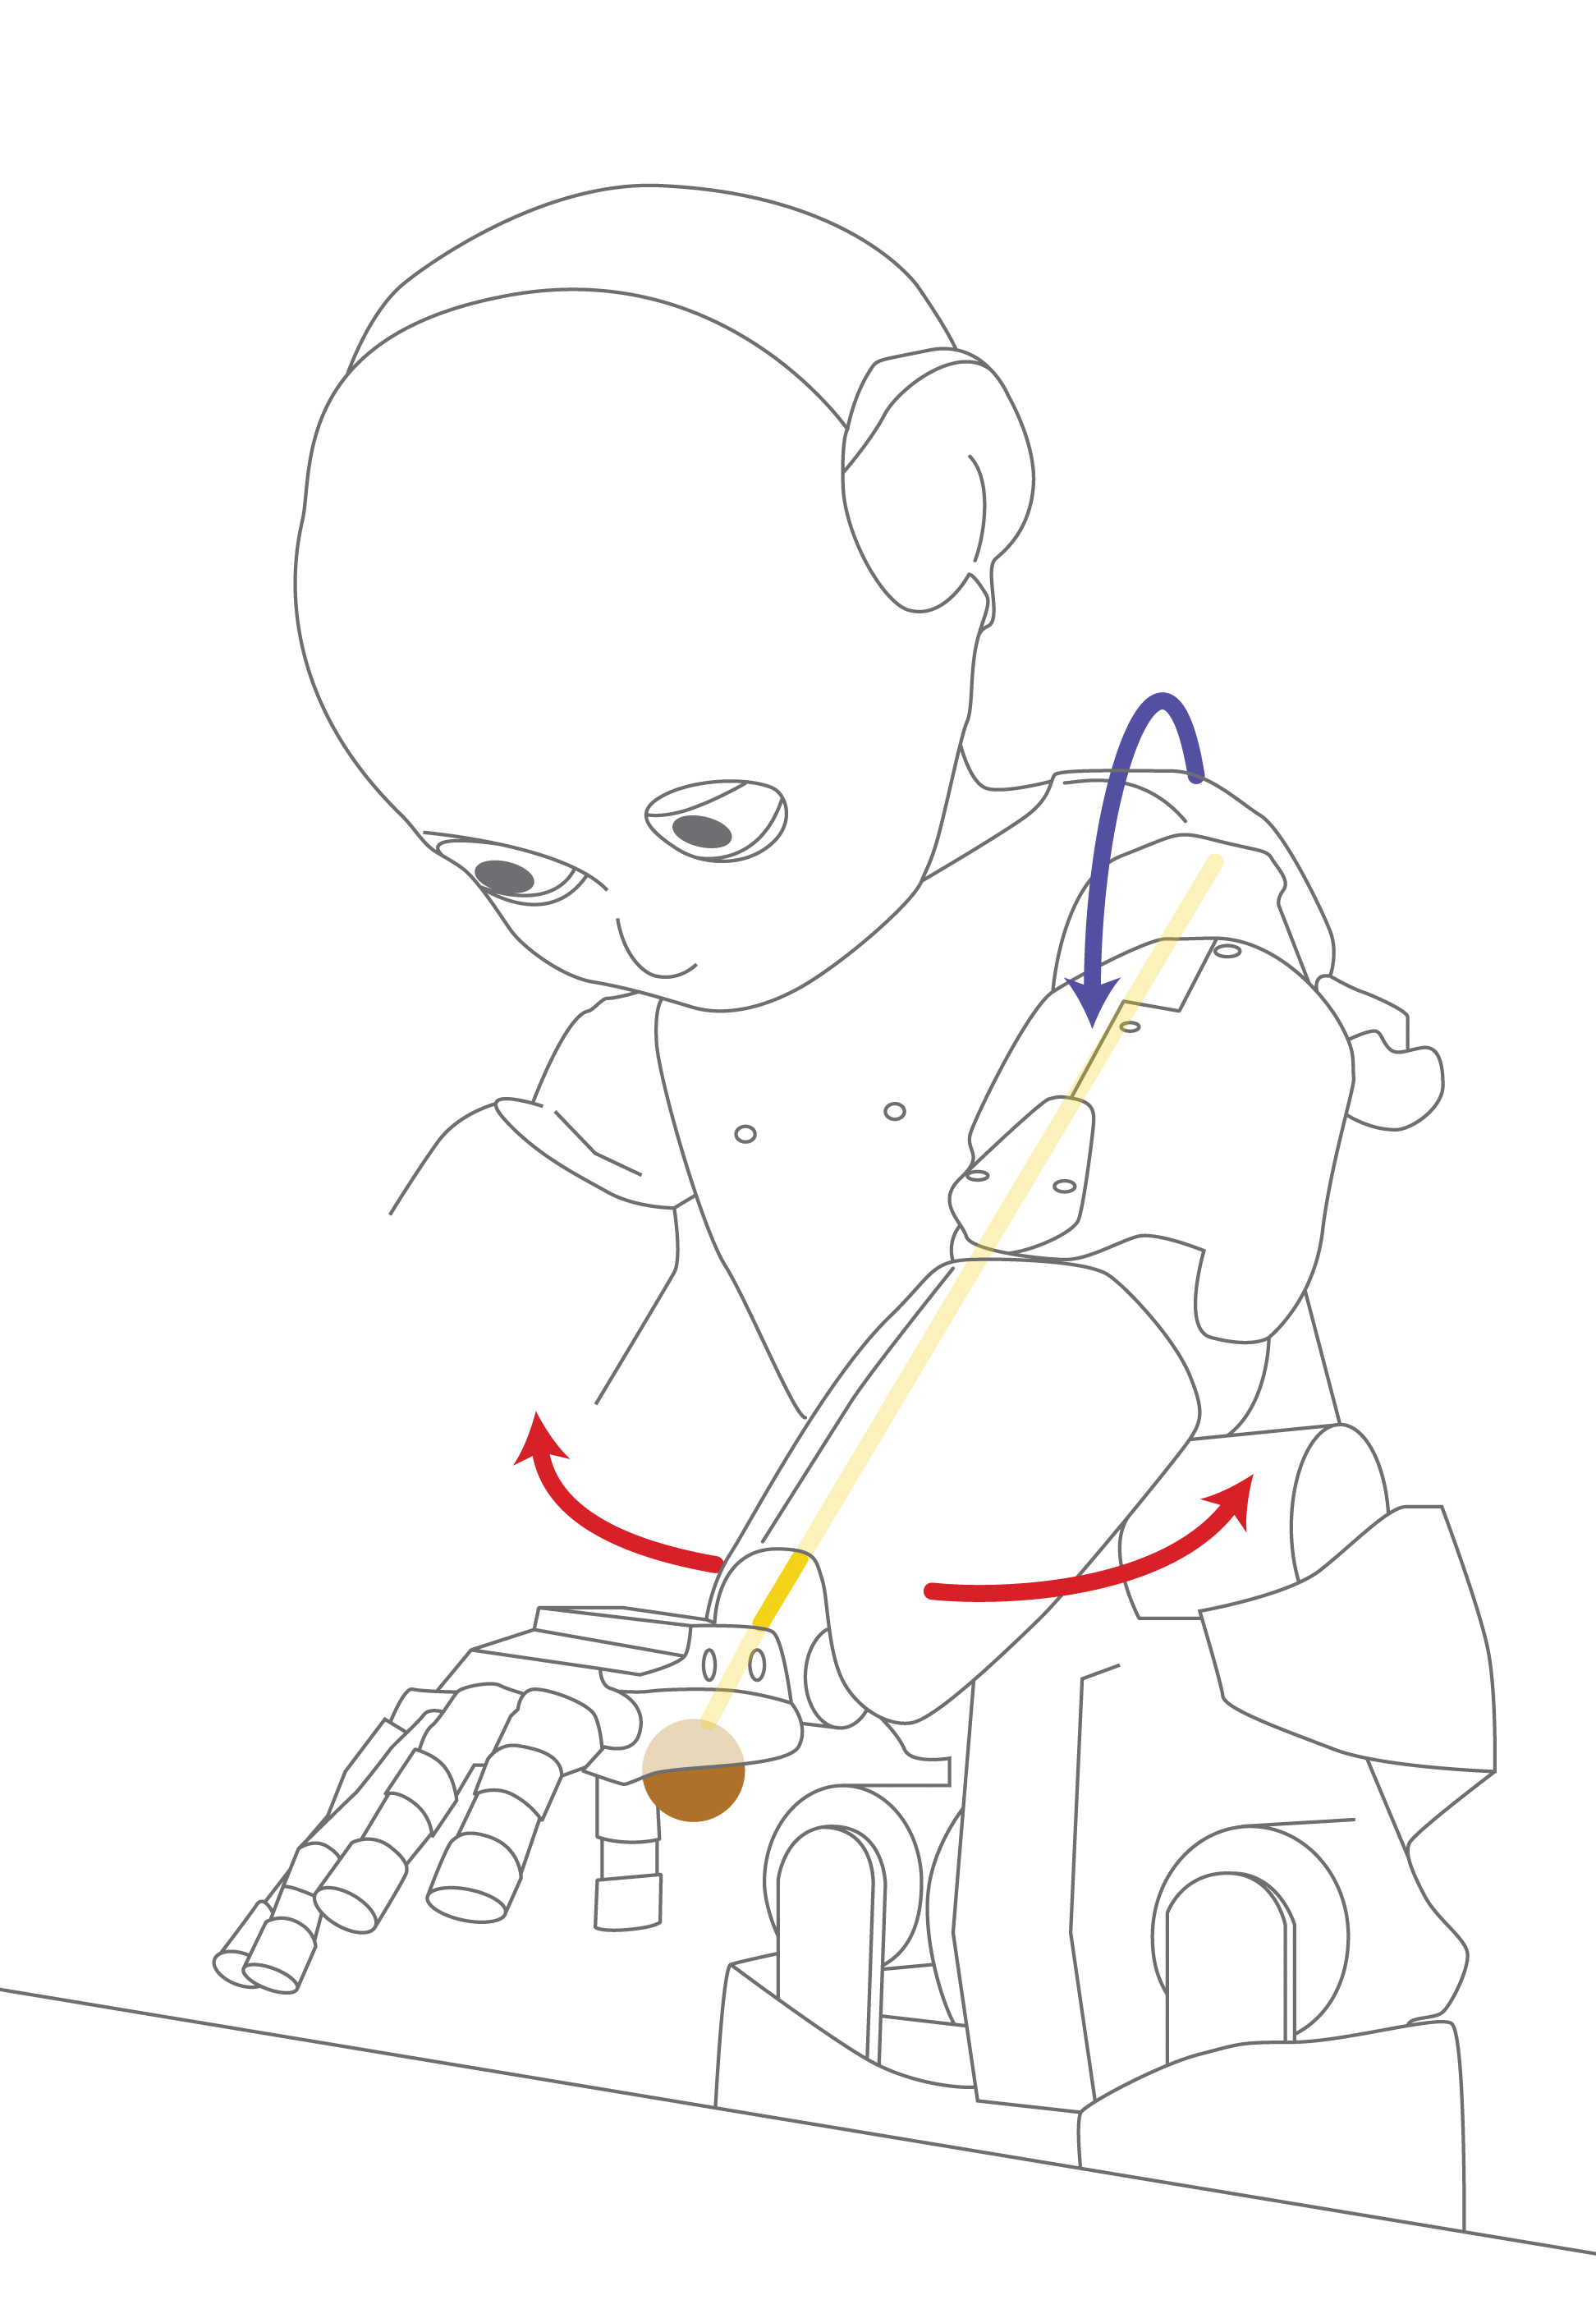
\includegraphics[width=34mm]{icubWiimoteKinematic.png}}
	  %\subfloat[\ac{DPad} control.]{\label{fig:wiiCursorControl}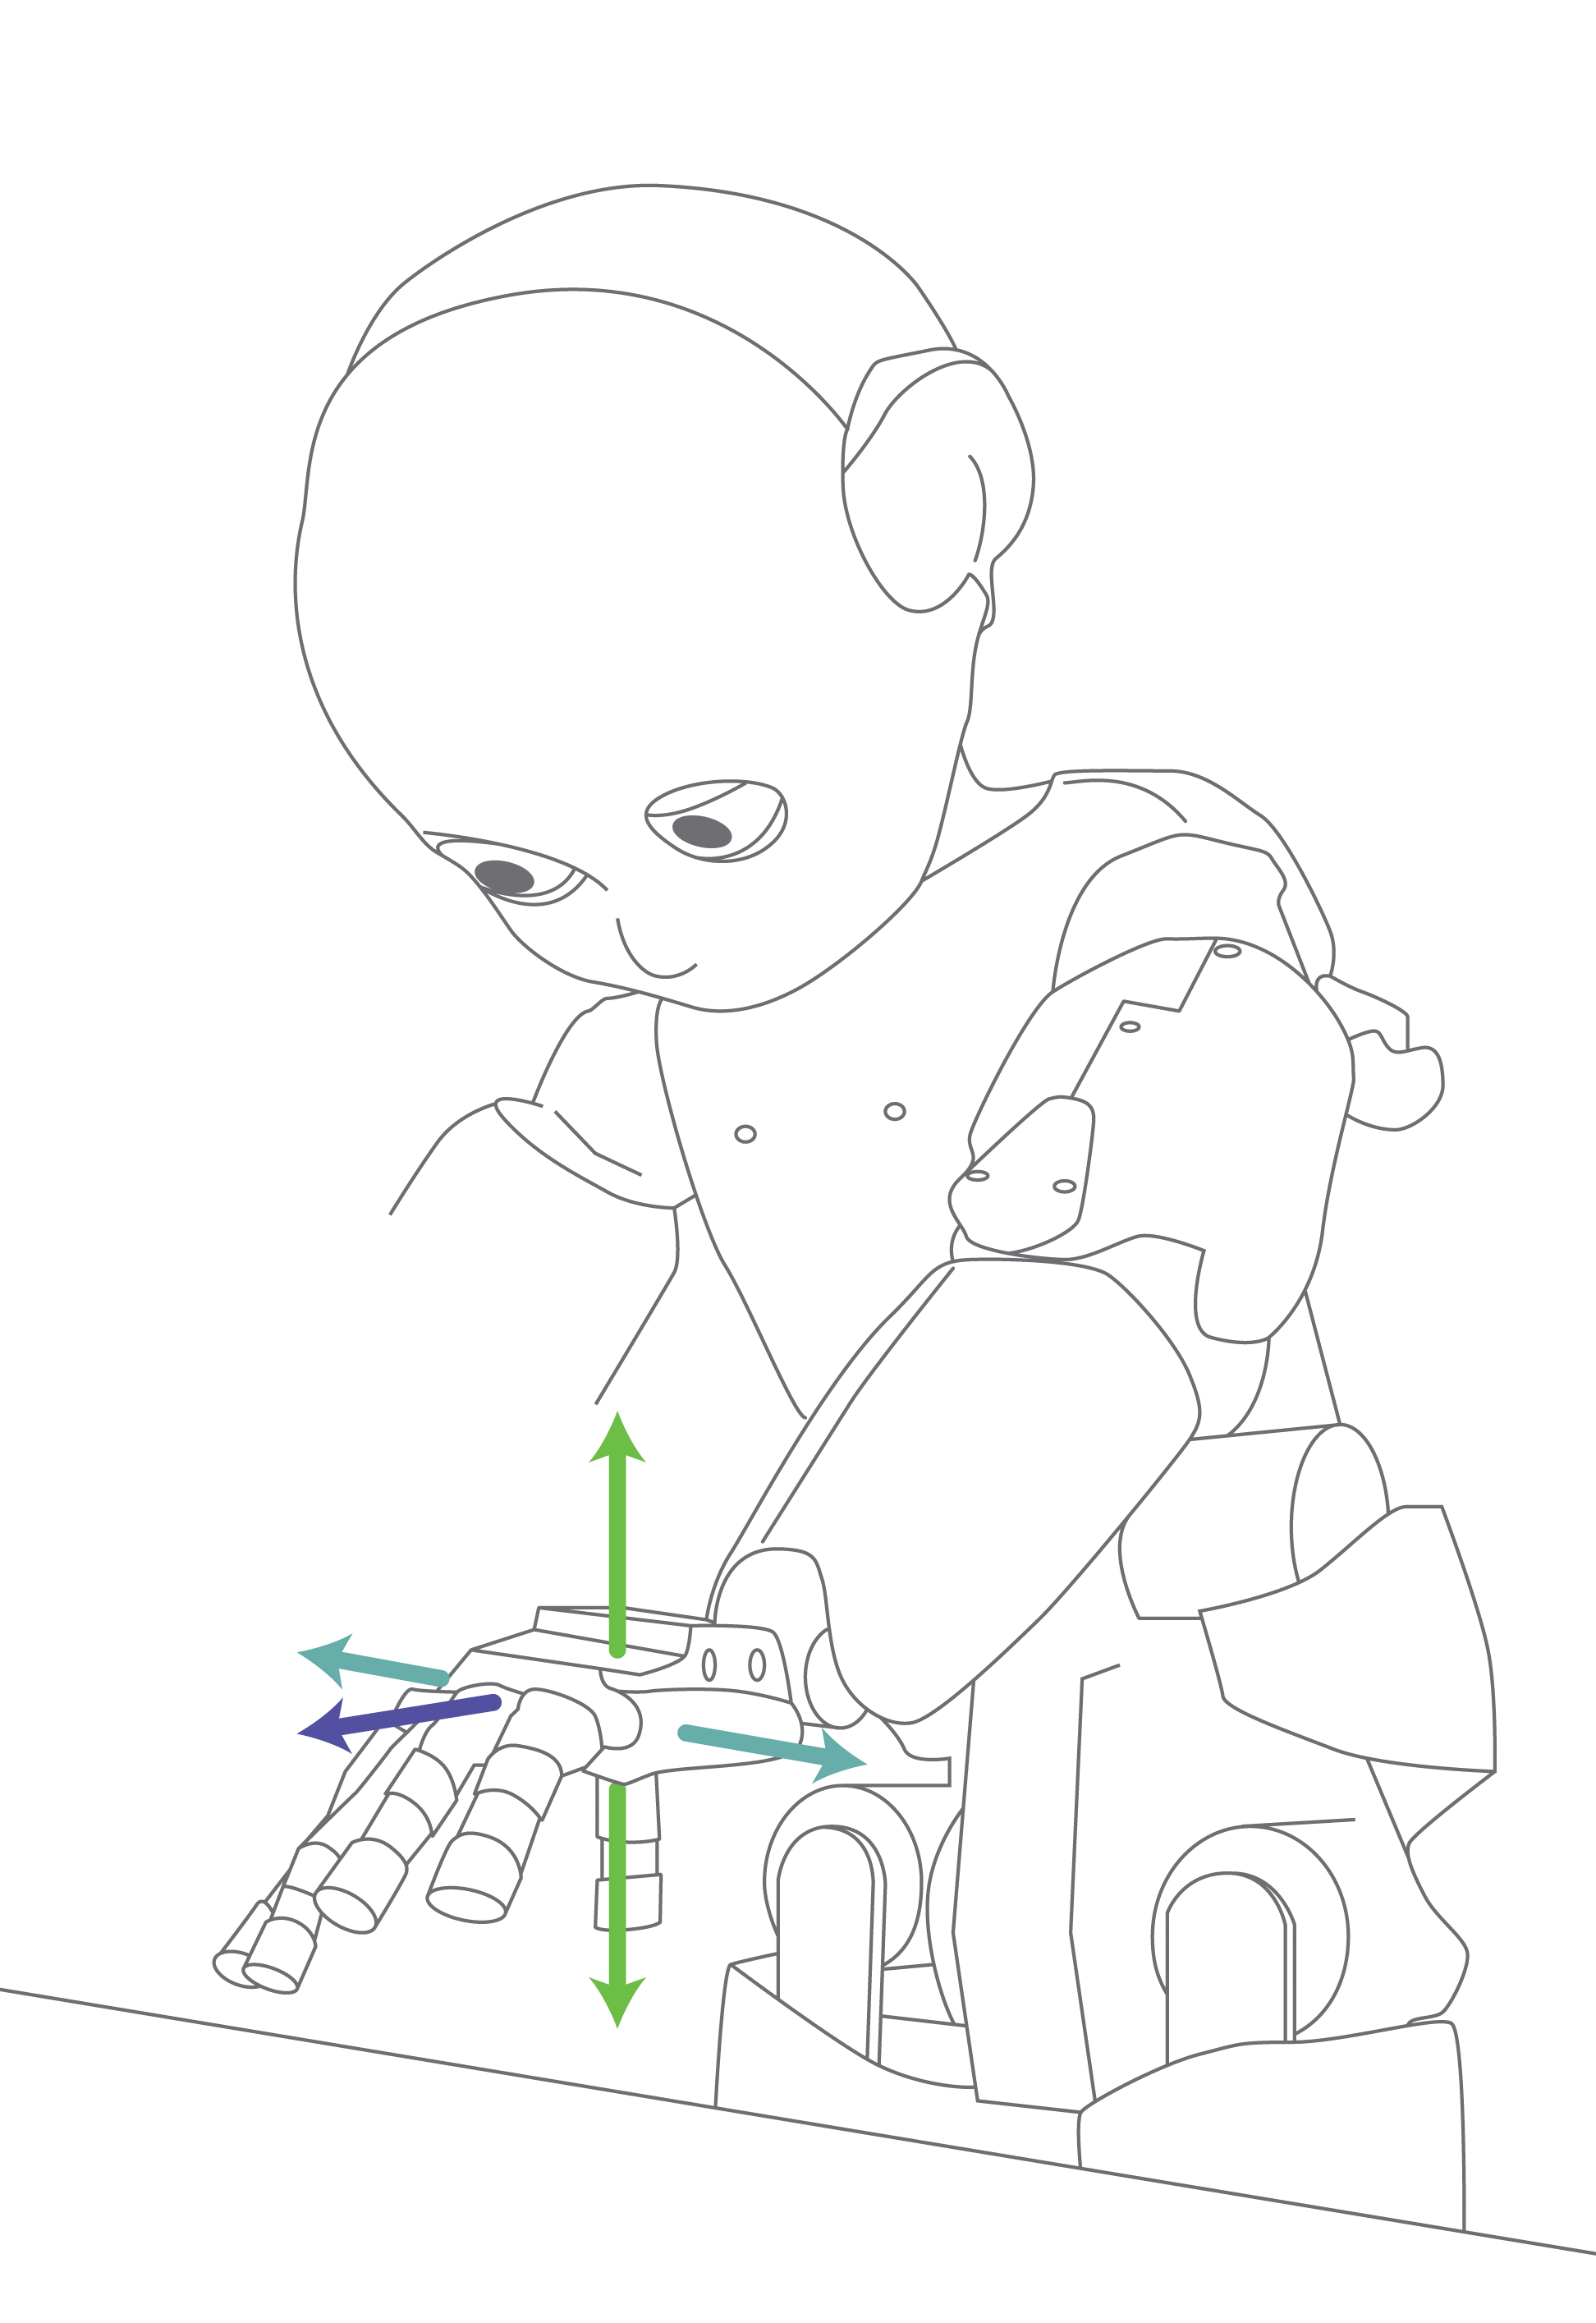
\includegraphics[width=27mm]{icubWiimoteCursor.png}}
	\caption{\ac{Wiimote} control types.} 
	\label{fig:wiimoteControl}
	\end{figure}
	
	The Kinect motor control maps the skeleton detected to the iCub motors. Figure \ref{fig:kinectSkeletonDetection} shows the skeleton detection made by a sample program. To map the skeleton detected by the Kinect to the iCub each of the rotation matrices that define the skeleton is converted to Euler angles, if its confidence level is higher than a defined threshold. The Euler angles are mapped to the motors directly depending on the motor axis. This way a pose that is detected by the Kinect is mimicked by the iCub in the most similar way possible.
	
	The Kinect kinematic control maps the user hand position to the iCub end-effector. Figure \ref{fig:kinectHandDetection} shows the hand detection made by a sample program. The metaphor used for this interaction is grabbing the robot hand, while standing face to face with it. So the iCub will follow the user hand detected by the Kinect, in a mirrored way. Pushing the hand front will mean for the iCub to pull the hand towards itself. Moving the hand to the left, will mean moving the hand to the right relatively to the iCub origin. The iCub only moves relatively to the hand initial position, where the initial position is the position of the hand on the first moment the \ac{Wiimote} button is pressed.

	\begin{figure}[htb]
	\centering
	  \subfloat[Kinect hand detection.]{\label{fig:kinectHandDetection}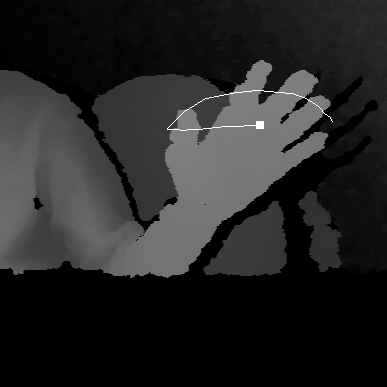
\includegraphics[width=34mm]{CaptureKinectHandSquare.png}}
  \hspace{5mm}
	  \subfloat[Kinect skeleton detection.] {\label{fig:kinectSkeletonDetection}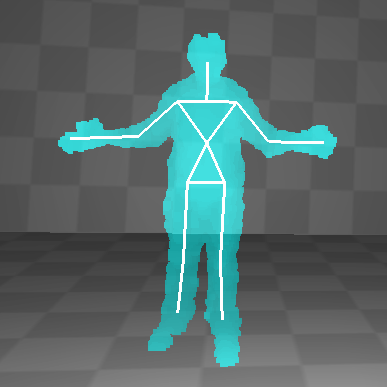
\includegraphics[width=34mm]{CaptureKinectSkeletonSquare.png}}
	\caption{Kinect detection made by sample programs.} 
	\label{fig:kinectDetection}
	\end{figure}